% -*- coding: utf-8 -*-
%-------------------------designed by zcf--------------
\documentclass[UTF8,a4paper,10pt]{ctexart}
\usepackage[left=3.17cm, right=3.17cm, top=2.74cm, bottom=2.74cm]{geometry}
\usepackage{amsmath}
\usepackage{graphicx,subfig}
\usepackage{float}
\usepackage{cite}
\usepackage{pgfplots}
\usepackage{background}
\usepackage{caption}
\usepackage{enumerate}
\usepackage{booktabs} %表格
\usepackage{multirow}
\usepackage{pdfpages}
\usepackage{tikz}
\usepackage{tikz-qtree}
\newcommand{\tabincell}[2]{\begin{tabular}{@{}#1@{}}#2\end{tabular}}  %表格强制换行
%-------------------------字体设置--------------
% \usepackage{times} 
\usepackage{ctex}
\setCJKmainfont[ItalicFont=Noto Sans CJK SC Bold, BoldFont=Noto Serif CJK SC Black]{Noto Serif CJK SC}
\newcommand{\yihao}{\fontsize{26pt}{36pt}\selectfont}           % 一号, 1.4 倍行距
\newcommand{\erhao}{\fontsize{22pt}{28pt}\selectfont}          % 二号, 1.25倍行距
\newcommand{\xiaoer}{\fontsize{18pt}{18pt}\selectfont}          % 小二, 单倍行距
\newcommand{\sanhao}{\fontsize{16pt}{24pt}\selectfont}  %三号字
\newcommand{\xiaosan}{\fontsize{15pt}{22pt}\selectfont}        % 小三, 1.5倍行距
\newcommand{\sihao}{\fontsize{14pt}{21pt}\selectfont}            % 四号, 1.5 倍行距
\newcommand{\banxiaosi}{\fontsize{13pt}{19.5pt}\selectfont}    % 半小四, 1.5倍行距
\newcommand{\xiaosi}{\fontsize{12pt}{18pt}\selectfont}            % 小四, 1.5倍行距
\newcommand{\dawuhao}{\fontsize{11pt}{11pt}\selectfont}       % 大五号, 单倍行距
\newcommand{\wuhao}{\fontsize{10.5pt}{15.75pt}\selectfont}    % 五号, 单倍行距
%-------------------------章节名----------------
\usepackage{ctexcap} 
\CTEXsetup[name={,、},number={ \chinese{section}}]{section}
\CTEXsetup[name={(,)},number={\chinese{subsection}}]{subsection}
\CTEXsetup[name={,.},number={\arabic{subsubsection}}]{subsubsection}
%-------------------------页眉页脚--------------
\usepackage{fancyhdr}
\pagestyle{fancy}
\lhead{\kaishu \leftmark}
% \chead{}
\rhead{\kaishu 并行程序设计实验报告}%加粗\bfseries 
\lfoot{}
\cfoot{\thepage}
\rfoot{}
\renewcommand{\headrulewidth}{0.1pt}  
\renewcommand{\footrulewidth}{0pt}%去掉横线
\newcommand{\HRule}{\rule{\linewidth}{0.5mm}}%标题横线
\newcommand{\HRulegrossa}{\rule{\linewidth}{1.2mm}}
%-----------------------伪代码------------------
\usepackage{algorithm}  
\usepackage{algorithmicx}  
\usepackage{algpseudocode}  
\floatname{algorithm}{Algorithm}  
\renewcommand{\algorithmicrequire}{\textbf{Input:}}  
\renewcommand{\algorithmicensure}{\textbf{Output:}} 
\usepackage{lipsum}  
\makeatletter
\newenvironment{breakablealgorithm}
  {% \begin{breakablealgorithm}
  \begin{center}
     \refstepcounter{algorithm}% New algorithm
     \hrule height.8pt depth0pt \kern2pt% \@fs@pre for \@fs@ruled
     \renewcommand{\caption}[2][\relax]{% Make a new \caption
      {\raggedright\textbf{\ALG@name~\thealgorithm} ##2\par}%
      \ifx\relax##1\relax % #1 is \relax
         \addcontentsline{loa}{algorithm}{\protect\numberline{\thealgorithm}##2}%
      \else % #1 is not \relax
         \addcontentsline{loa}{algorithm}{\protect\numberline{\thealgorithm}##1}%
      \fi
      \kern2pt\hrule\kern2pt
     }
  }{% \end{breakablealgorithm}
     \kern2pt\hrule\relax% \@fs@post for \@fs@ruled
  \end{center}
  }
\makeatother
%------------------------代码-------------------
\usepackage{xcolor} 
\usepackage{listings}
\lstset{ 
breaklines,%自动换行
basicstyle=\small,
escapeinside=``,
keywordstyle=\color{ blue!70} \bfseries,
commentstyle=\color{red!50!green!50!blue!50},% 
stringstyle=\ttfamily,% 
extendedchars=false,% 
linewidth=\textwidth,% 
numbers=left,% 
numberstyle=\tiny \color{blue!50},% 
frame=trbl% 
rulesepcolor= \color{ red!20!green!20!blue!20} 
}
%------------超链接----------
\usepackage[colorlinks,linkcolor=black,anchorcolor=blue]{hyperref}
%------------------------TODO-------------------
\usepackage{enumitem,amssymb}
\newlist{todolist}{itemize}{2}
\setlist[todolist]{label=$\square$}
% for check symbol 
\usepackage{pifont}
\newcommand{\cmark}{\ding{51}}%
\newcommand{\xmark}{\ding{55}}%
\newcommand{\done}{\rlap{$\square$}{\raisebox{2pt}{\large\hspace{1pt}\cmark}}\hspace{-2.5pt}}
\newcommand{\wontfix}{\rlap{$\square$}{\large\hspace{1pt}\xmark}}
%------------------------水印-------------------
\usepackage{tikz}
\usepackage{xcolor}
\usepackage{eso-pic}

\newcommand{\watermark}[3]{\AddToShipoutPictureBG{
\parbox[b][\paperheight]{\paperwidth}{
\vfill%
\centering%
\tikz[remember picture, overlay]%
  \node [rotate = #1, scale = #2] at (current page.center)%
    {\textcolor{gray!80!cyan!30!magenta!30}{#3}};
\vfill}}}



%———————————————————————————————————————————正文———————————————————————————————————————————————
%----------------------------------------------
\begin{document}
\ttfamily
\backgroundsetup{scale=0.5, angle=0, opacity = 0.1, contents = {
\includegraphics[width=\paperwidth, height=\paperwidth, keepaspectratio]{back.png}}}
\begin{titlepage}
    \begin{center}
    
\includegraphics[width=0.8\textwidth]{pics/NKU.jpg}\\[1cm]    
    \textsc{\Huge \kaishu{\textbf{南\ \ \ \ \ \ 开\ \ \ \ \ \ 大\ \ \ \ \ \ 学}} }\\[0.9cm]
    \textsc{\huge \kaishu{\textbf{计\ \ 算\ \ 机\ \ 学\ \ 院}}}\\[0.5cm]
    \textsc{\Large \textbf{编译系统原理工程作业}}\\[0.8cm]
    \HRule \\[0.9cm]
    { \LARGE \bfseries 预备工作2——定义你的编译器\&汇编编程}\\[0.4cm]
    \HRule \\[2.0cm]
    \centering
    \textsc{\LARGE \kaishu{辛紫遇\ 王晓凡}}\\[0.5cm]
    \textsc{\LARGE \kaishu{年级\ :\ 2019级}}\\[0.5cm]
    \textsc{\LARGE \kaishu{专业\ :\ 计算机科学与技术\ 信息安全}}\\[0.5cm]
    \textsc{\LARGE \kaishu{指导教师\ :\ 王刚}}\\[0.5cm]
    \vfill
    {\Large \today}
    \end{center}
\end{titlepage}
%-------------摘------要--------------
\newpage
\thispagestyle{empty}
\renewcommand{\abstractname}{\kaishu \sihao \textbf{摘要}}
    \begin{abstract}
        本文使用上下文无关文法描述了我们需要实现的编译器所支持的SysY语言特性,用该语言设计了一系列能够尽可能多体现语言特性程序,编写了等价的ARM汇编程序并测试。

        \noindent  %顶格
        \textbf{\\\ 关键字:SysY,CFG,ARM汇编}\textbf{} \\\ \\\
    \end{abstract}
%----------------------------------------------------------------
\tableofcontents
%----------------------------------------------------------------
\newpage
\setcounter{page}{1}

\section{引言}
    1983年,ANSI为C语言创立了一套标准,即ANSI C。这套标准经历了C89,C90,C99和C11四个阶段,几乎被所有广泛使用的编译器支持。
    ANSI C包括关键字,基础数据类型,结构类型,数组,指针,字符串,运算符号,控制语句,函数和输入输出等特性。
    在本课程中,我们将仿照特性这些实现它的一个子集--SysY语言。
    
\section{SysY语言的CFG描述}
    一个完善有效的语言应当被使用上下文无关文法描述。我们将参照SysY语言定义,自底向上地组织起整个语言。由于字体难以排版,本文使用单引号引起所有终结符。

    \subsection{标识符}
    标识符应该由字母或下划线引起,后面跟随一系列字母、数字或下划线。
    \begin{lstlisting}
      id -> nondigit
           | id nondigit
           | id digit
nondigit -> 'A'|'B'|'C'|'D'|'E'|'F'|'G'|'H'|'I'|'J'|'K'|'L'|'M'
           |'N'|'O'|'P'|'Q'|'R'|'S'|'T'|'U'|'V'|'W'|'X'|'Y'|'Z'
           |'a'|'b'|'c'|'d'|'e'|'f'|'g'|'h'|'i'|'j'|'k'|'l'|'m'
           |'n'|'o'|'p'|'q'|'r'|'s'|'t'|'u'|'v'|'w'|'x'|'y'|'z'
           |'_'
   digit -> '0'|'1'|'2'|'3'|'4'|'5'|'6'|'7'|'8'|'9'
    \end{lstlisting}

    \subsection{数值常量}
    数值常量可以为十进制数、0引起的八进制数、0x或0X引起的十六进制数。
    \begin{lstlisting}
    int-const -> dec-const | oct-const | hex-const
    dec-const -> nonzero-digit | dec-const digit
    oct-const -> 0 | oct-const oct-digit
    hex-const -> hex-prefix hex-digit | hex-const hex-digit
   hex-prefix -> '0x' | '0X'
nonzero-digit -> '1'|'2'|'3'|'4'|'5'|'6'|'7'|'8'|'9'
    oct-digit -> '0'|'1'|'2'|'3'|'4'|'5'|'6'|'7'
    hex-digit -> '0'|'1'|'2'|'3'|'4'|'5'|'6'|'7'|'8'|'9'
                |'a'|'b'|'c'|'d'|'e'|'f'
                |'A'|'B'|'C'|'D'|'E'|'F'
    \end{lstlisting}

    \subsection{数据类型}
    变量只有整数类型,函数返回值可以有整数或空类型。
    \begin{lstlisting}
   BType -> 'int'
FuncType -> 'void' | 'int'
    \end{lstlisting}

    \subsection{运算符}
    运算符分为三个优先级,从低到高分别为加减运算符、乘除取模运算符、单目运算符。
    \begin{lstlisting}
  AddOp -> '+' | '−'
  MulOp -> '*' | '/' | '%'
UnaryOp -> '+' | '−' | '!'
   EqOp -> '==' | '!='
  RelOp -> '<' | '>' | '<=' | '>='
    \end{lstlisting}
    
    \subsection{算数表达式}
    算数表达式分为一般算数表达式和常量表达式,优先级与运算符一致。
    函数调用被认为是一个单目表达式。
    还需要定义括号表达式和合法左值表达式。
    \begin{lstlisting}
        Exp -> AddExp
   ConstExp -> AddExp (仅当所有id均为常量时)
     AddExp -> MulExp | AddExp AddOp MulExp
     MulExp -> UnaryExp | MulExp MulOp UnaryExp
   UnaryExp -> PrimaryExp | UnaryOp UnaryExp
             | id '()' | id '(' FuncRParams ')'
FuncRParams -> Exp | FuncRParams ',' Exp
 PrimaryExp -> '(' Exp ')' | LVal | int-const
       LVal -> id | id '[' Exp ']'
  ConstLVal -> id | id '[' ConstExp ']'
    \end{lstlisting}

    \subsection{条件表达式}
    条件表达式的优先级从低到高为:或表达式、与表达式、相等不等表达式、关系表达式。
    \begin{lstlisting}
   Cond -> LOrExp
 LOrExp -> LAndExp | LOrExp '||' LAndExp
LAndExp -> EqExp | LAndExp '&&' EqExp
  EqExp -> RelExp | EqExp EqOp RelExp
 RelExp -> AddExp | RelExp RelOp AddExp
    \end{lstlisting}

    \subsection{语句}
    语句分为赋值语句、分号语句、表达式语句、if语句、if-else语句、while语句、break、continue、return语句。
    语句块也被视为一个语句。
    多个声明和语句被花括号包括即成为语句块。
    声明又分为常量声明和变量声明。
    \begin{lstlisting}
     Block -> '{' BlockItems '}'
BlockItems -> BlockItem | BlockItems BlockItem
 BlockItem -> Decl | Stmt
      Decl -> ConstDecl | VarDecl
      Stmt -> LVal '=' Exp ';'
            | ';' | Exp ';' | Block
            | 'if' '( Cond ')' Stmt
            | 'if' '( Cond ')' Stmt 'else' Stmt
            | 'while' '(' Cond ')' Stmt
            | 'break' ';' | 'continue' ';'
            | 'return' ';' | 'return' Exp ';'
    \end{lstlisting}

    \subsection{常量声明语句}
    声明语句需要考虑是否为常量声明。
    一个声明语句可以声明多个变量,每个声明都可赋初值,数组初值可以由花括号引起。
    \begin{lstlisting}
    ConstDecl -> 'const' BType ConstDefs ';'
    ConstDefs -> ConstDef | ConstDefs ',' ConstDef
     ConstDef -> ConstLVal '=' ConstInitVal
 ConstInitVal -> ConstExp | '{' '}' | '{' ConstInitVals '}'
ConstInitVals -> ConstInitVal | ConstInitVals ',' ConstInitVal
    \end{lstlisting}

    \subsection{变量声明语句}
    \begin{lstlisting}
 VarDecl -> BType VarDefs ';'
 VarDefs -> VarDef | VarDefs ',' VarDef
  VarDef -> ConstLVal | ConstLVal '=' InitVal
 InitVal -> Exp | '{' '}' | '{' InitVals '}'
InitVals -> InitVal | InitVals ',' InitVal
    \end{lstlisting}

    \subsection{函数定义}
    函数定义由类型、函数名、参数表和函数体组成,参数可以有0个或多个。
    \begin{lstlisting}
    FuncDef -> FuncType id '(' ')' Block
             | FuncType id '(' FuncFParams ')' Block
FuncFParams -> FuncFParam | FuncFParams ',' FuncFParam
 FuncFParam -> BType id | BType id '[' ']'
             | FuncFParam '[' Exp ']'
    \end{lstlisting}

    \subsection{编译单元}
    在最顶层,所有的声明和函数定义被集成为编译单元。
    \begin{lstlisting}
CompUnit -> Unit | CompUnit Unit
    Unit -> Decl | FuncDef
    \end{lstlisting}

\section{样例程序}
    我们根据上一节定义的语言设计了一段代码,并力求其能全面地包含尽可能多的语言特性:
    \begin{lstlisting}[title=SysY语言样例程序, frame=trbl, language={C}]
#include "sylib.h"

int i, j=101;

void doNothing(){
    int k = 1;
    0;;
    return;
}

int func(int x, int y){
    if(x != y) return 5;
    else {
        doNothing();
        return 6;
    }
}

int main(){
    int a[2][2] = {{0, 1}, {}}; // 0 1 0 0
    const int b = -9+5*2; // 1
    while(!(0 && b <= 5)){ // true
        a[1][b] = func(7, 8); // 0 1 0 5
        if(a[0][0] || b==0) continue; // false
        break;
    }
    putarray(4, a); // 0 1 0 5
    putint(b); // 1
    return 0;
}
    \end{lstlisting}

    将这段代码编写成等价的ARM汇编代码:
    \begin{lstlisting}[title=ARM汇编样例程序, frame=trbl}]
    .arch	armv7-a
    .arm
    .file	"test.c"
    @ 以下是代码段
    .text

    @ i是全局变量,但没有初始化,所以我们放在.bss段
    .globl	i
    .bss

    @ 保持内存对齐
    .align	2
    
    @ i是我们int实例出来的一个对象,因此是object类型,又因为int是4字节,因此i的size为4
    .type	i, %object
    .size	i, 4

    @ 上面只是通知汇编器我们定义的i是个什么变量,我们还需要给i以内存空间
i:
    .space	4

    @ j是初始化的全局变量,我们放在.data段,同时,因为j的大小是4字节(一个字),我们于是用.word给j赋值;其余的跟i一样
    .globl	j
    .data
    .align	2
    .type	j, %object
    .size	j, 4
j:
    .word	101

    @ 以下是代码段
    .text
    @ 声明下面的代码段是一个函数
    .align	1
    .globl	doNothing
    .type	doNothing, %function
doNothing:
    push	{lr,fp}	@ 这里我们压栈保存返回地址和栈基地址
    add	fp, sp, #0	@ 提升fp指向sp
    sub	sp, sp, #4	@ 扩栈,留下4字节大小的栈空间(因为只要这么多)

    mov		r4, #1			@ r4存放我们的局部变量k,因为r4是局部变量寄存器
    str		r4, [sp, #4]	@ 这里我们把变量k放到内存中存储,注意是r7(fp)+4的位置,

    nop				@ 注意,这里很有趣,我们源文件这里是"0;;",但是毫无意义,因此被翻译为空指令

    add		sp, #4			@ 回收之前的栈空间
    pop		{fp}				@ 弹栈,将之前保存的值返还回去
    pop		{lr}

    bx	lr			@ lr寄存器记录着返回地址,现在我们返回去
    .size	doNothing, .-doNothing

    .align	1
    .globl	func
    .type	func, %function
func:
    push	{lr, fp}
    add	fp, sp, #0
    @ 注意这里我们不需要扩栈了,因为没有新建变量

    @ 注意,在arm汇编中是从左至右一次放入r0,r1,r2,r3中的,例如这里调用func(x,y),r0存储x,r1存储y
    cmp		r0, r1
    beq		.LABLE_of_func
    mov		r0, #5						@ 返回值放在r0
    b		.LABLE_return_of_func		@ 这两句相当于return 5;
.LABLE_of_func:
    bl		doNothing(PLT)				@ 因为这是汇编代码,还没分配具体的内存,因此不知道函数所在的内存地址;同时,目前操作系统规定代码段不能修改,因此均采用PLT表作为跳转,
                                        @ 这样我们编写汇编代码时就不需要关心函数的具体位置或偏移,只需要标注一下让汇编器自动往对应的PLT项跳转即可

    mov		r0, #6
.LABLE_return_of_func:
    pop		{fp}
    pop		{lr}
    bx   lr								@ 这次我们没有使用栈,就不用恢复栈了,把保存的值恢复出来即可
    .size	func, .-func

    .align	1
    .globl	main
    .type	main, %function
main:
    push	{lr, fp}
    add	fp, sp, #0
    sub	sp, sp, #20   @ 准备20的空间,因为我们有a[2][2]共16字节+ const int b 共4字节

    @ 局部变量a[2][2]的空间位于sp+4到sp+16的位置,从低地址向高地址增长
    mov r0, #0
    str r0, [sp, #4]		@ a[0][0] = 0
    str r0, [sp, #12]		@ a[1][0] = 0
    str r0, [sp, #16]		@ a[1][1] = 0
    mov r0, #1
    str r0, [sp, #8]		@ a[0][1] = 1

    @ 局部变量 const int b 存储于栈顶,我们可以看到先声明的变量放在高地址,后声明的变量放在低地址
    @ gcc给出的汇编是直接复制公式结果了,我们这里为体现过程要去计算
    mov r0, #5
    mov r1, #2
    mul r3, r1, r0		@ 计算5*2
    add r0, r3, #-9		@ 计算-9+5*2
    str r0, [sp]		@ const int b = -9+5*2

    @ 我们进入了while循环
.LABLE_WHILE_LOOP:
    @ 这一步代码的意思是:我们设置r0为b是否小于等于5的flag,若小于等于5,则r0为1,否则为0
    mov r0, #1
    ldr r1, [sp]
    cmp r1, #5
    bls .LABLE_not_set_flag 
    mov r0, #0
.LABLE_not_set_flag:
    
    and r0, r0, #0		@ 等价于0&&b<=5
    mvn r0, r0
    and r0, r0, #1      @ 这两步等价于!(0&&b<=5)
    cmp r0, #1
    bne .LABLE_END_LOOP @ 这里注意一下,在源程序中我们可以直接算出表达式的结果是1,因此while条件总是执行的,但这里我们为了体现计算条件表达式这一过程,我们设计如上“冗余”的代码
    
    mov r1, #8
    mov r0, #7
    bl	func(PLT)
    mov r1, #2
    mov r2, #1
    mul r1, r2, r1		@ r1 = 2*1
    ldr r2, [sp]		@ r2 = b
    add r1, r1, r2      @ r1 = 2*1 + b, 这里我们的目的是获得a[1][b]的偏移量,因为a一行两个元素,故1*2,又因为在b列,故1*2+b
    lsl r1, r1, #2      @ r1 = 4*(2*1+b), r1左移两位即r1乘4,之所以要乘四是因为a中每个元素都是int,占4个字节

    add r1, #4			@ 因为a的地址在sp+4的位置,所以r1要加4
    str r0, [sp, r1]	@ a[1][b] = r0 = func(7,8)
    ldr r0, [sp, #4]	@ r0 = a[0][0]
    
    ldr r1, [sp]			@ r1 = b
    cmp r1, #0
    mrs r1, cpsr
    and r1, r1, #0x40000000	@ 这步操作是为了获取b==0的布尔值结果,去掉其它结果,cmp指令的比较结果会写到cpsr寄存器的zero flag上,若相等则为1,不等则为0
    lsr r1, #30				@ 因为zero flag在第31位,所以要逻辑右移30位,得到结果:r1 = (b == 0)

    orr r0, r0, r1			@ 计算 a[0][0] || (b == 0)
    cmp r0, #0
    bgt .LABLE_WHILE_LOOP	@ 如果(a[0][0] || (b == 0))为真,则continue
    nop						@ 否则,直接break;因为我们这里是直接退出循环并不做任何操作,所以我们直接一个nop表示break;语句

.LABLE_END_LOOP:
    add r1, sp, #4		@ r1 = a的地址
    mov r0, #4
    bl	putarray(PLT)   @ 调用putarray()

    ldr r0, [sp]		@ r0 = b
    bl	putint(PLT)		@ 调用putint()

    mov r0, #0			@ return 0; r0存储函数返回值
    add sp, sp, #20		@ 回收栈空间

    pop		{fp}
    pop		{lr}
    bx   lr				@ 返回
    
    .size	main, .-main
    .ident	"GCC: (Ubuntu 9.3.0-17ubuntu1~20.04) 9.3.0"
    .section	.note.GNU-stack,"",%progbits
    \end{lstlisting}

    运行这段汇编代码,结果如下:
    \begin{figure}[H]
        \centering
        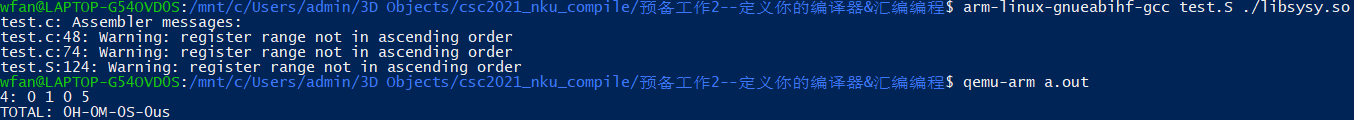
\includegraphics[width=14cm]{pics/pic.png}
        \caption{汇编代码运行结果}
        \label{fig:pic}
    \end{figure}

\section{总结}
    \subsection{分工情况}
    辛紫遇负责CFG设计、SysY语言程序设计、文档编写、汇编代码微调,
    王晓凡负责汇编代码编写与测试、文档修改。

    \subsection{Gitlab链接}
    \href{https://gitlab.eduxiji.net/Wang\_XiaoFan/csc2021\_nku\_compile}{https://gitlab.eduxiji.net/Wang\_XiaoFan/csc2021\_nku\_compile}

\end{document}
